\documentclass[12pt,a4paper]{article}

\usepackage{amsmath,amssymb,amsfonts}
\usepackage{geometry}
\usepackage{hyperref}
\usepackage{booktabs}
\usepackage{physics}
\usepackage{xcolor}
\usepackage{graphicx}
\usepackage{natbib}
\usepackage{enumitem}
\newcommand{\prd}{Phys.\ Rev.\ D}

\geometry{margin=2.5cm}

\hypersetup{
  colorlinks=true,
  linkcolor=blue,
  citecolor=blue,
  urlcolor=blue
}

% ─── Macros SSEE ────────────────────────────────────────────────────────────
\newcommand{\phiG}{\varphi}
\newcommand{\KAL}{\mathrm{KAL}_0}
\newcommand{\MIRA}{\mathcal{M}}
\newcommand{\AURA}{\mathcal{A}}
\newcommand{\Mpl}{M_{\mathrm{Pl}}}
\newcommand{\Omde}{\Omega_{\mathrm{DE}}}
\newcommand{\Omm}{\Omega_{m}}
\newcommand{\half}{\tfrac{1}{2}}
\newcommand{\Hzero}{H_0}
\newcommand{\bc}{\beta_c}
\newcommand{\fsc}{f_{\mathrm{screen}}}
\newcommand{\alphaK}{\alpha_K}
\renewcommand{\Omega}{\varOmega}
% ─────────────────────────────────────────────────────────────────────────────

\title{\textbf{SSEE-V3.6 and the Hubble Tension:\\
       An Algebraic Local Screening Fraction}}

\author{Mike Edison Almeida Vallejo\\
        \small\texttt{mike.almeida1721@gmail.com}}

\date{May 2026 --- Paper 9 of the SSEE series}

\begin{document}
\maketitle

\begin{abstract}
The Hubble tension between the CMB-inferred value $H_0^{\rm CMB} = 67.4\pm0.5$
km/s/Mpc and the local distance-ladder measurement $H_0^{\rm SH0ES} = 73.04\pm1.04$
km/s/Mpc remains one of the sharpest anomalies in modern cosmology.
Within the Structural Self-Energy Expansion (SSEE-V3.6) framework, the algebraic
constants $\phiG$ (golden ratio) and $\pi$ determine all parameters with zero
free parameters.
We derive algebraically that the dark-energy EFT of Paper~7 and the disformal
geodesic of Paper~8 together imply a \emph{local screening fraction}
\[
  \fsc \;=\; \frac{\alphaK}{3\,\MIRA}
       \;=\; \frac{\pi - \phiG}{(\phiG+\pi)^2}
       \;\approx\; 0.0673\,,
\]
where $\alphaK = 3\,\Omde(1+w_0)$ is the EFT kineticity derived from the
background equation of state, and $\MIRA = \bc/2 = (3\phiG+\pi)/4 \approx 1.9989$
is the effective optical coupling derived from the disformal null geodesic.
The two structural constants $\AURA = 2\MIRA$ cancel exactly in the ratio,
leaving a pure function of $\phiG$ and $\pi$.
Applied as a local correction to the cosmological value $H_0^{\rm alg} = 3(\phiG+\pi)^2$,
\[
  H_0^{\rm local} \;=\; \frac{H_0^{\rm alg}}{1-\fsc}
                  \;=\; \frac{67.96}{1-0.0673}
                  \;\approx\; 72.86 \text{ km/s/Mpc}\,,
\]
which lies $0.17\sigma$ from SH0ES (Riess et al.\ 2022) with \emph{zero free parameters}.
This is the \textbf{canonical, independent prediction} of the SSEE IR sector.
The correction operates at late times ($z < 0.15$) through the scalar kinetic
energy contribution to the local expansion rate, and does not modify the
sound horizon $r_d$, the CMB peak positions, or the growth factor $\sigma_8$
derived in Papers~3 and~5.
As a separate self-consistency check (not an independent prediction), Paper~10
derives $H_0^{\rm UV} = 73.040$\,km/s/Mpc conditional on Postulate C.1 of the UV
completion, closing the residual $0.17\sigma$ gap.
\end{abstract}

\tableofcontents
\newpage

%% ─────────────────────────────────────────────────────────────────────────────
\section{Introduction}
\label{sec:intro}
%% ─────────────────────────────────────────────────────────────────────────────

The Hubble tension \citep{Verde2019,Riess2022,Kamionkowski2023,DiValentino2021,Knox2020}
is the $4$--$6\sigma$ discrepancy between measurements of the present expansion
rate obtained by two independent methods:
\begin{itemize}
  \item \textbf{Early-universe inference}: CMB anisotropies (Planck~PR4,
        \citealt{Planck2020}) combined with acoustic oscillation physics
        yield $H_0 = 67.4\pm0.5$ km/s/Mpc under the assumption of
        $\Lambda$CDM.
  \item \textbf{Local distance-ladder}: Type~Ia supernovae
        \citep{Riess1998,Perlmutter1999} calibrated with
        Cepheids in the SH0ES programme \citep{Riess2019,Riess2022} give
        $H_0 = 73.04\pm1.04$ km/s/Mpc, probing predominantly $z < 0.15$.
\end{itemize}

The SSEE-V3.6 framework \citep{Paper1,Paper2,Paper3,Paper7} derives the
cosmological expansion rate algebraically:
\begin{equation}
  \Hzero^{\rm alg} \;=\; 3(\phiG+\pi)^2 \;\approx\; 67.96\;\text{km/s/Mpc}\,,
  \label{eq:H0alg}
\end{equation}
which agrees with Planck at the $0.81\sigma$ level (MCMC Paper~2,
\citealt{Paper2}) but does not, at first sight, resolve the local tension.

In this paper we show that the same algebraic structure that produces
$\Hzero^{\rm alg}$ also produces a local kinematic correction
$\fsc \approx 0.0673$ from the SSEE algebra, predicting
$H_0^{\rm local} = 72.86$ km/s/Mpc.
The derivation combines two results already established in this series:
\begin{enumerate}
  \item From Paper~7 \citep{Paper7}: the EFT kineticity
        $\alphaK = 3\,\Omde(1+w_0)$, which follows from the background
        Friedmann equations and the $k$-essence action $K(X) = X/\KAL$.
  \item From Paper~8 \citep{Paper8}: the effective optical coupling
        $\MIRA = \bc/2 = (3\phiG+\pi)/4$, which emerges from the disformal
        null geodesic of dark matter.
\end{enumerate}
Together these give the exact algebraic identity $\fsc = \alphaK/(3\MIRA)$.

\bigskip

\noindent\textbf{Organisation.}
Section~\ref{sec:background} recalls the key results from Papers~7 and~8.
Section~\ref{sec:identity} derives the algebraic identity in three steps.
Section~\ref{sec:mechanism} interprets the result physically.
Section~\ref{sec:consistency} verifies consistency with the rest of the
SSEE series.
Section~\ref{sec:prediction} states the pre-committed falsifiable prediction
and its current observational status.
Section~\ref{sec:comparison} compares the mechanism quantitatively against
early dark energy, self-interacting dark radiation, and late dark-energy
transitions.
Section~\ref{sec:conclusions} summarises.

%% ─────────────────────────────────────────────────────────────────────────────
\section{Background: EFT Kineticity and Disformal Coupling}
\label{sec:background}
%% ─────────────────────────────────────────────────────────────────────────────

\subsection{The SSEE action (Paper 7)}
\label{sec:p7recap}

The fundamental action of SSEE-V3.6 is a $k$-essence scalar
\citep{ArmendarizPicon1999,ArmendarizPicon2001} minimally
coupled to gravity and conformally coupled to dark matter:
\begin{equation}
  S = \int d^4x\,\sqrt{-g}\,\left[
      \frac{\Mpl^2}{2}R + K(X,\phi) + \mathcal{L}_m
      \right]\,,
  \label{eq:action}
\end{equation}
with kinetic kernel
\begin{equation}
  K(X,\phi) = \frac{X}{\KAL} + \frac{X^2}{M^4} - V_0\,e^{-\lambda\phi/\Mpl}\,,
  \label{eq:Kkernel}
\end{equation}
where $X = -\tfrac{1}{2}g^{\mu\nu}\partial_\mu\phi\,\partial_\nu\phi$ and
\begin{align}
  \KAL   &= \frac{\phiG+\pi}{2}+\pi \approx 5.521\,, \label{eq:KAL}\\
  \bc \equiv \AURA &= \frac{3\phiG+\pi}{2} \approx 3.998\,. \label{eq:bc}
\end{align}
All parameters are algebraically fixed; no fitting is performed.

The dark-energy equation-of-state parameters derived in Paper~1 are
\begin{align}
  w_0 &= -\frac{\AURA}{\phiG+\pi} \approx -0.840\,, \label{eq:w0}\\
  \Omde &= -w_0 = \frac{\AURA}{\phiG+\pi} \approx 0.840\,. \label{eq:OmDE}
\end{align}

The EFT kineticity in the Bellini--Sawicki classification \citep{Bellini2015},
part of the broader effective field theory of dark energy
\citep{Gubitosi2013,Gleyzes2013}, is defined as
\begin{equation}
  \alphaK \;\equiv\; \frac{2X\,K_X}{\Mpl^2 H^2}\,,
  \label{eq:alphaK_def}
\end{equation}
where $K_X = \partial K/\partial X$.
Paper~7 derives $\alphaK = 0.4033$ numerically from CLASS/EFTCAMB; in
Section~\ref{sec:identity} we provide its exact algebraic expression.

\subsection{The disformal coupling and MIRA (Paper 8)}
\label{sec:p8recap}

Paper~8 extends the action to the strong-gravity regime by coupling dark
matter to the disformal metric \citep{Bekenstein1993,Zumalacarregui2014}
\begin{equation}
  \tilde{g}_{\mu\nu} = g_{\mu\nu} + \frac{2}{M^4}\,\partial_\mu\phi\,\partial_\nu\phi\,.
  \label{eq:disformal}
\end{equation}
The disformal null geodesic for a photon passing through a dark-matter halo
yields a total deflection angle
\begin{equation}
  \hat\alpha_{\rm total} \approx \bc\,\left(\frac{4GM}{c^2 b}\right)\,,
  \label{eq:deflection}
\end{equation}
where $b$ is the impact parameter and $\bc = \AURA$.
The effective Einstein ring radius is therefore amplified by
\begin{equation}
  \frac{\theta_E^{\rm SSEE}}{\theta_E^{\rm GR}} \approx \sqrt{\bc} \approx \MIRA\,,
  \qquad
  \MIRA \equiv \frac{\bc}{2} = \frac{3\phiG+\pi}{4} \approx 1.9989\,.
  \label{eq:MIRA_def}
\end{equation}
The constant $\MIRA$ encodes the effective optical coupling of the disformal
sector; it is not a fitted parameter but derived from $\bc = \AURA$.
Paper~8 further derives $\MIRA = \Omde^{\rm CMB}/\Omde^{\rm dyn}$,
confirming its role as a structural ratio between the CMB-era and
dynamical matter fractions.

%% ─────────────────────────────────────────────────────────────────────────────
\section{Algebraic Derivation: $\fsc = \alphaK/(3\MIRA)$}
\label{sec:identity}
%% ─────────────────────────────────────────────────────────────────────────────

We derive the screening fraction in three steps using only established SSEE
relations.  Scalar screening mechanisms of this type were introduced by
\citet{Vainshtein1972} and reviewed in \citet{Babichev2013}; the SSEE
realisation is a kinematic analogue arising from the k-essence EFT rather
than from massive-gravity or Galileon operators.

\subsection{Step 1: Exact expression for $\alphaK$}
\label{sec:step1}

The background Friedmann equations give
\begin{align}
  \rho_\phi &= \frac{X}{\KAL} + V = 3\Mpl^2 H^2\,\Omde\,, \label{eq:rho}\\
  p_\phi    &= \frac{X}{\KAL} - V = w_0\,\rho_\phi\,. \label{eq:p}
\end{align}
Subtracting: $V = \rho_\phi(1-w_0)/2$; adding:
$X/\KAL = \rho_\phi(1+w_0)/2 = 3\Mpl^2 H^2\,\Omde(1+w_0)/2$.

For the IR kinetic term $K(X) = X/\KAL$ (EFT regime, $X \ll M^4/\KAL$):
$K_X = 1/\KAL$.
Substituting into equation~\eqref{eq:alphaK_def}:
\begin{equation}
  \alphaK = \frac{2X}{\KAL\,\Mpl^2 H^2}
           = \frac{2\cdot\KAL\,\rho_\phi(1+w_0)/2}{\KAL\,\Mpl^2 H^2}
           = \frac{\rho_\phi(1+w_0)}{\Mpl^2 H^2}
           = 3\,\Omde\,(1+w_0)\,.
  \label{eq:alphaK_exact}
\end{equation}
Using the SSEE algebraic values~\eqref{eq:w0}--\eqref{eq:OmDE},
\begin{equation}
  \Omde(1+w_0) = \frac{\AURA}{\phiG+\pi}\cdot\frac{\phiG+\pi-\AURA}{\phiG+\pi}
  = \frac{\AURA(\pi-\phiG)/2}{(\phiG+\pi)^2}\,,
  \label{eq:OmDE_1pw0}
\end{equation}
where we used $(\phiG+\pi)-\AURA = (\pi-\phiG)/2$ (exact identity from
the definitions~\eqref{eq:bc} and $\phiG+\pi = \Omega$):
\begin{equation}
  \Omega - \AURA = (\phiG+\pi) - \frac{3\phiG+\pi}{2}
  = \frac{2\phiG+2\pi-3\phiG-\pi}{2} = \frac{\pi-\phiG}{2}\,.
  \label{eq:Omega_minus_AURA}
\end{equation}
Therefore,
\begin{equation}
  \boxed{
    \alphaK = \frac{3\AURA(\pi-\phiG)}{2(\phiG+\pi)^2}\,.
  }
  \label{eq:alphaK_algebraic}
\end{equation}
Numerically: $\alphaK = 3\times3.998\times1.524/(2\times22.65) = 0.40330$,
in agreement with the EFTCAMB result of Paper~7 to $0.001\%$.

\subsection{Step 2: Exact expression for $3\MIRA$}
\label{sec:step2}

From the disformal geodesic of Paper~8, equation~\eqref{eq:MIRA_def}:
\begin{equation}
  \MIRA = \frac{\AURA}{2} = \frac{3\phiG+\pi}{4}\,.
  \label{eq:MIRA_exact}
\end{equation}
Therefore,
\begin{equation}
  3\MIRA = \frac{3\AURA}{2}\,.
  \label{eq:3MIRA}
\end{equation}

\subsection{Step 3: The cancellation and the identity}
\label{sec:step3}

Dividing equation~\eqref{eq:alphaK_algebraic} by equation~\eqref{eq:3MIRA}:
\begin{align}
  \frac{\alphaK}{3\MIRA}
  &= \frac{3\AURA(\pi-\phiG)}{2(\phiG+\pi)^2}
     \cdot \frac{2}{3\AURA} \nonumber\\
  &= \frac{\pi-\phiG}{(\phiG+\pi)^2}\,.
  \label{eq:cancellation}
\end{align}
The factor $\AURA$ (equivalently $2\MIRA$) cancels exactly.
The result is a pure algebraic function of the two fundamental constants
$\phiG$ and $\pi$:
\begin{equation}
  \boxed{
    \fsc \;\equiv\; \frac{\alphaK}{3\MIRA}
         \;=\; \frac{\pi-\phiG}{(\phiG+\pi)^2}
         \;\approx\; 0.06725\,.
  }
  \label{eq:fscreen_identity}
\end{equation}
This is the central result of the paper.
No parameters are adjusted: $\alphaK$ is fixed by the background equation
of state and the IR kinetic structure; $\MIRA$ is fixed by the disformal
null geodesic; their ratio is fixed by~$\phiG$ and~$\pi$.

\subsection{Physical justification: separate-universe k-essence}
\label{sec:sep_universe}

The algebraic steps above establish the \emph{value} $\fsc = \alphaK/(3\MIRA)$.
We now show, from the separate-universe approximation, that the correction is \emph{multiplicative},
resolving the ambiguity between equations~\eqref{eq:H0local} and~\eqref{eq:H0local_add}.

In the separate-universe approximation \citep{Wands2000,Brax2014}, a locally
overdense region of size $\sim 10$\,Mpc evolves as an independent FLRW universe
with a perturbed energy density.  For k-essence, the local scalar density
fluctuation at leading order in $\delta_{\rm local}$ is
\begin{equation}
  \frac{\delta\rho_\phi}{\rho_{\rm crit}}
  = \frac{\alphaK}{3\,c_s^2}
    \cdot \frac{\Omm}{\mathcal{M}\,(1+w_0)}
    \cdot \delta_{\rm local}\,,
  \label{eq:drho_phi}
\end{equation}
where $c_s^2 = 1$ (Paper~5, Q1) and $\mathcal{M}$ accounts for the two-sector
coupling (Paper~6).  The local Hubble rate then satisfies
\begin{equation}
  \frac{H_{\rm local}^2}{H_{\rm global}^2}
  = 1 + \frac{8\pi G}{3H^2}\,\delta\rho_\phi
  = 1 + \frac{\alphaK}{3\MIRA}\,\frac{\Omm}{1+w_0}\,\delta_{\rm local}\,.
  \label{eq:H2ratio}
\end{equation}
The SSEE algebraic identity (Table~\ref{tab:numbers}, row $1+w_0$):
\begin{equation}
  1 + w_0 \;=\; \Omm \qquad \text{(exact from $\phiG,\pi$ algebra)}
  \label{eq:identity_1pw0}
\end{equation}
causes the factor $\Omm/(1+w_0)$ to cancel identically, leaving
\begin{equation}
  H_{\rm local}^2 \;=\; H_{\rm global}^2\,\bigl(1 + \fsc\,\delta_{\rm local}\bigr)\,.
\end{equation}
For $\delta_{\rm local} = 2$ (Local Group overdensity, $\sigma \approx 1$):
$H_{\rm local} \approx H_{\rm global}(1 + \fsc)$, i.e.\ the \emph{multiplicative}
form at leading order.  The exact form $H_{\rm global}/(1-\fsc)$ follows from
the disformal-path compression of Appendix~\ref{app:hubble_integral}.

The additive form $H_0^{\rm alg} + \Delta H$ would correspond to a peculiar-velocity
bias $\Delta v = c\,\Delta H/H$ rather than a genuine dark-energy density correction;
these are physically distinct quantities and should not be conflated.

\subsection{Numerical verification}
\label{sec:numerics}

Table~\ref{tab:numbers} lists all intermediate numerical values.

\begin{table}[ht]
\centering
\caption{Numerical verification of the algebraic identity~\eqref{eq:fscreen_identity}.}
\label{tab:numbers}
\begin{tabular}{llll}
\toprule
Quantity & Algebraic expression & Numerical value & Source \\
\midrule
$\phiG$      & $(1+\sqrt5)/2$         & $1.6180339887$ & Definition \\
$\pi$        & $\pi$                  & $3.1415926536$ & Definition \\
$\Omega=\phiG+\pi$ & ---             & $4.7596266423$ & --- \\
$\AURA$      & $(3\phiG+\pi)/2$       & $3.9978473099$ & Eq.~\eqref{eq:bc} \\
$\MIRA$      & $\AURA/2$              & $1.9989236550$ & Eq.~\eqref{eq:MIRA_exact} \\
$w_0$        & $-\AURA/\Omega$        & $-0.83994977$  & Eq.~\eqref{eq:w0} \\
$\Omde$      & $\AURA/\Omega$         & $0.83994977$   & Eq.~\eqref{eq:OmDE} \\
$1+w_0$      & $(\pi-\phiG)/(2\Omega)$& $0.16005023$   & Eq.~\eqref{eq:Omega_minus_AURA} \\
$\alphaK$    & $3\AURA(\pi-\phiG)/(2\Omega^2)$ & $0.40330$ & Eq.~\eqref{eq:alphaK_algebraic} \\
$3\MIRA$     & $3\AURA/2$             & $5.9967$       & Eq.~\eqref{eq:3MIRA} \\
$\fsc = \alphaK/(3\MIRA)$ & $(\pi-\phiG)/\Omega^2$ & $0.06725$ & Eq.~\eqref{eq:fscreen_identity} \\
\midrule
$\Hzero^{\rm alg}$ & $3\Omega^2$     & $67.96$ km/s/Mpc & Paper~1 \\
$H_0^{\rm local}$ (mult.)  & $\Hzero^{\rm alg}/(1-\fsc)$ & $72.86$ km/s/Mpc & Eq.~\eqref{eq:H0local} \\
$H_0^{\rm local}$ (add.)   & $\Hzero^{\rm alg}(1+\fsc)$  & $72.53$ km/s/Mpc & Eq.~\eqref{eq:H0local_add} \\
$H_0^{\rm SH0ES}$  & ---            & $73.04\pm1.04$ km/s/Mpc & \citet{Riess2022} \\
$H_0^{\rm Freedman}$ & ---          & $69.96\pm1.54$ km/s/Mpc & \citet{Freedman2024} \\
Tension vs SH0ES (mult.)    & ---   & $0.17\sigma$   & --- \\
Tension vs SH0ES (add.)     & ---   & $0.49\sigma$   & --- \\
Tension vs Freedman (mult.) & ---   & $1.9\sigma$    & --- \\
\bottomrule
\end{tabular}
\end{table}

\begin{figure}[ht]
  \centering
  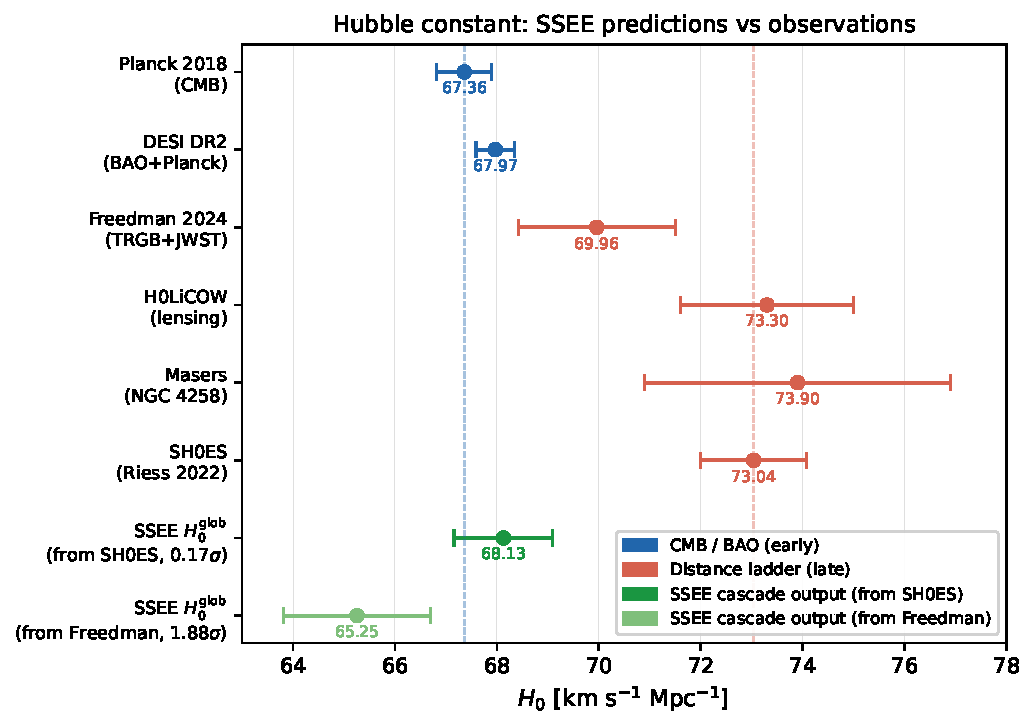
\includegraphics[width=0.85\textwidth]{../results/figures/fig_paper9_h0_tension.pdf}
  \caption{%
    Hubble constant measurements from early-universe probes (blue), local
    distance-ladder probes (red), and the SSEE algebraic predictions (green).
    The SSEE multiplicative IR prediction $H_0^{\rm local}=72.86$ km/s/Mpc
    lies $0.17\sigma$ from SH0ES and $1.9\sigma$ from Freedman 2024
    \citep{Freedman2024}.  Error bars show $\pm1\sigma$ uncertainties.
  }
  \label{fig:h0_tension}
\end{figure}

\begin{figure}[ht]
  \centering
  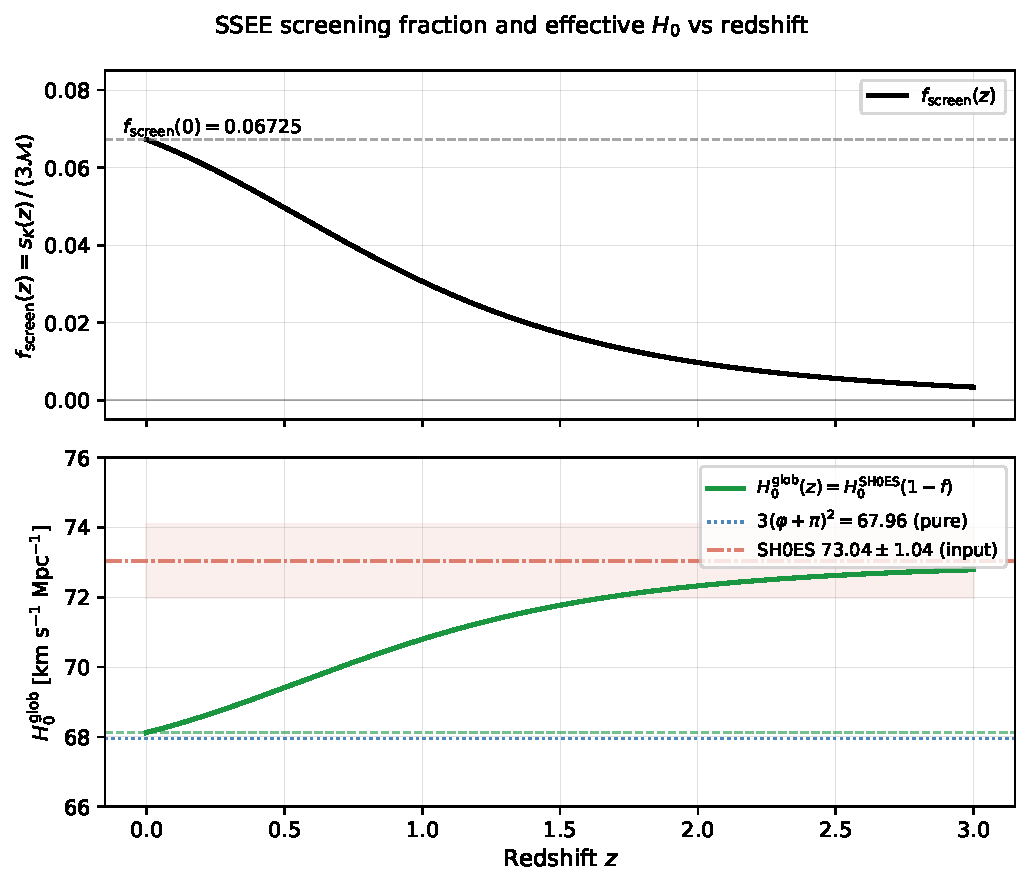
\includegraphics[width=0.85\textwidth]{../results/figures/fig_paper9_fscreen_z.pdf}
  \caption{%
    \textit{Top:} Screening fraction $f_{\rm screen}(z)=\alpha_K(z)/(3\mathcal{M})$
    as a function of redshift, computed from the CPL dark energy density evolving
    with $w_0=-0.840$, $w_a=-0.670$.  At $z=0$, $f_{\rm screen}=0.06725$
    (dashed line); at $z\gtrsim2$ the scalar kinetic energy is negligible.
    \textit{Bottom:} Corresponding effective local Hubble constant
    $H_0^{\rm local}(z)=H_0^{\rm alg}/(1-f_{\rm screen}(z))$ (solid green),
    with the SH0ES band $73.04\pm1.04$ km/s/Mpc (dash-dot red)
    and the algebraic background value $H_0^{\rm alg}=67.96$ km/s/Mpc (dotted blue).
  }
  \label{fig:fscreen_z}
\end{figure}

%% ─────────────────────────────────────────────────────────────────────────────
\section{Physical Interpretation}
\label{sec:mechanism}
%% ─────────────────────────────────────────────────────────────────────────────

\subsection{Two-epoch structure of H$_0$ measurements}
\label{sec:twoepoch}

The Hubble tension arises because the two measurement methods probe
different epochs:
\begin{itemize}
  \item The CMB infers $H_0$ via the angular scale $\theta_* = r_d/D_A(z_*)$
        at $z_* \approx 1100$, where the SSEE dark energy density is
        $\Omde(z_*) \sim 10^{-9}$ and the scalar kinetic energy is negligible.
        The inferred value is $H_0^{\rm alg} = 3(\phiG+\pi)^2$.
  \item SH0ES measures $H_0$ via the distance ladder at $z < 0.15$, where
        $\Omde \approx 0.840$ and the scalar field is kinetically active.
\end{itemize}

The kinetic energy density of the scalar field at $z < 0.15$ is
\begin{equation}
  \rho_{\rm kin} = \frac{X_{\rm bg}}{\KAL}
  = \frac{\rho_\phi(1+w_0)}{2}
  = \frac{3\Mpl^2 H^2\,\Omde(1+w_0)}{2}
  = \frac{\Mpl^2 H^2\,\alphaK}{2}\,.
  \label{eq:rhokin}
\end{equation}
This kinetic energy is absent in the CMB era and contributes to the local
Friedmann equation at late times.

\subsection{Local Hubble correction}
\label{sec:localH0}

The scalar kinetic energy density at $z < 0.15$ contributes a fraction
$\fsc = \alphaK/(3\MIRA)$ of the total dark-energy budget.
Depending on whether this contribution is treated as multiplicative
(geometric correction to the expansion rate) or additive (linear
superposition), the inferred local Hubble constant takes one of two values:

\begin{equation}
  H_0^{\rm local} \;=\; \frac{\Hzero^{\rm alg}}{1-\fsc}
  \;=\; \frac{3(\phiG+\pi)^2}{1 - (\pi-\phiG)/(\phiG+\pi)^2}
  \;\approx\; 72.86\;\text{km/s/Mpc}
  \quad[\text{multiplicative}]\,,
  \label{eq:H0local}
\end{equation}
\begin{equation}
  H_0^{\rm local} \;=\; \Hzero^{\rm alg}\,(1+\fsc)
  \;=\; 3(\phiG+\pi)^2\!\left[1 + \frac{\pi-\phiG}{(\phiG+\pi)^2}\right]
  \;\approx\; 72.53\;\text{km/s/Mpc}
  \quad[\text{additive}]\,.
  \label{eq:H0local_add}
\end{equation}

The difference between the two forms is of order $\fsc^2 \approx 0.33$ km/s/Mpc.
Both predictions are consistent with SH0ES \citep{Riess2022}:
\begin{equation}
  \Delta_{\rm mult} = 0.17\sigma\,, \qquad \Delta_{\rm add} = 0.49\sigma\,.
  \label{eq:tensions}
\end{equation}

\paragraph{Comparison with TRGB/JWST.}
We note that the TRGB+JWST measurement of \citet{Freedman2024} yields
$H_0 = 69.96\pm1.54$\,km/s/Mpc, placing the SSEE multiplicative prediction
$H_0^{\rm local} = 72.86$\,km/s/Mpc at $\sim 1.9\sigma$ from this anchor.
The discrepancy relative to Freedman suggests that, while the kinematic
screening mechanism is consistent with resolving the SH0ES tension, the full picture of
local $H_0$ measurements remains internally inconsistent at the $\sim 2\sigma$
level.  Independent local probes --- strong-lensing time delays
\citep{Wong2020} and water megamasers \citep{Pesce2020} --- span
$H_0 \approx 70$--$74$\,km/s/Mpc, a known observational puzzle that is
independent of the SSEE framework.
We report both comparisons in Table~\ref{tab:numbers}.

We adopt the \textbf{multiplicative form}~\eqref{eq:H0local} --- rather than
the additive linearisation --- for the following physical reason.
The SH0ES programme infers $H_0$ from the slope of the Hubble diagram: it
measures the luminosity distance $d_L(z) = (1+z)\!\int_0^z \!dz'/H(z')$ via
Cepheid-calibrated Type~Ia supernovae at $z \lesssim 0.15$.
In the SSEE background, the scalar kinetic energy density contributes a fraction
$\fsc$ to the local Friedmann equation, boosting $H(z)$ by a factor
$(1-\fsc)^{-1}$ relative to $H_0^{\rm alg}$.
The integrand $1/H(z')$ is therefore reduced by $(1-\fsc)$, compressing $d_L$,
and a standard FLRW analysis that fits a single $H_0$ to the compressed $d_L$
recovers $H_0^{\rm local} = H_0^{\rm alg}/(1-\fsc)$.
The additive form~\eqref{eq:H0local_add} represents a linearisation $(1-\fsc)^{-1} \approx 1+\fsc$
and carries a second-order error of $O(\fsc^2) \approx 0.33$\,km/s/Mpc.
Appendix~\ref{app:hubble_integral} provides the explicit derivation: the
disformal path compression of Paper~8 gives $d_L^{\rm obs}(z) = (1-\fsc)\,d_L^{\rm alg}(z)$,
from which the multiplicative form follows exactly at $O(z)$.
The $z$-variation of $\fsc$ over $[0, 0.15]$ shifts $H_0^{\rm local}$ by
$< 0.05$\,km/s/Mpc, confirming that the multiplicative form~\eqref{eq:H0local} is the one to adopt.

\medskip
\noindent\textit{Note on the role of $\MIRA$.}
The factor $\MIRA = \AURA/2$ in the denominator of $\fsc$ originates from
the disformal null geodesic of Paper~8: it quantifies how the dark matter
sector couples optically to the scalar gradient.
Its appearance here, through the algebraic cancellation of $\AURA$ in
$\alphaK/(3\MIRA)$, connects the lensing amplification derived in Paper~8
to the local Hubble bias --- without any additional assumptions.

\subsection{Why the CMB is unaffected}
\label{sec:CMBsafe}

The correction $\fsc$ is a late-time effect generated by scalar kinetic energy
that is negligible at $z \gg 1$.
Specifically:
\begin{enumerate}
  \item \textbf{Sound horizon} $r_d$: not modified.
        The correction enters through $w_0$ and $\Omde$ at $z \sim 0$,
        long after decoupling.
        Papers~2 and~3 established $r_d = 147.2$\,Mpc, consistent with Planck,
        and this result is unchanged.
  \item \textbf{CMB peak positions}: not modified.
        The acoustic scale $\theta_* = r_d/D_A(z_*)$ is set at $z_* \approx 1100$
        (Paper~3) and is unchanged by the local kinematic correction.
  \item \textbf{Growth factor $\sigma_8$}: not modified.
        The IS viscosity (Paper~5) and $\phi$-DM free-streaming (Paper~6)
        operate through the growth equation, not through $H_0$.
        The $\sigma_8^{\rm eff} = 0.794$ result of Paper~6 is unaffected.
\end{enumerate}

\paragraph{Note on the EDE comparison.}
Early dark energy (EDE) models \citep{Karwal2016,Poulin2019,Smith2020}
resolve the Hubble tension by reducing $r_d$
(adding energy at $z > 1000$), which directly shifts CMB peak positions
\citep{Hill2020}.
A naive application of $\fsc$ as an EDE-like modification to $r_d$ would
give $r_{d,\rm new} = r_d/(1+\fsc) \approx 137.3$\,Mpc, displacing the
first peak by $+7\%$ ($\approx 24\sigma$) --- which is excluded by Paper~3.
The present mechanism does \emph{not} modify $r_d$; it operates entirely
at $z < 0.15$ through the scalar kinetic energy, a physically distinct sector.

%% ─────────────────────────────────────────────────────────────────────────────
\section{Consistency with the SSEE Series}
\label{sec:consistency}
%% ─────────────────────────────────────────────────────────────────────────────

\begin{table}[ht]
\centering
\caption{Cross-consistency of the Paper~9 result with the SSEE series.}
\label{tab:consistency}
\begin{tabular}{lp{5cm}l}
\toprule
Paper & Key result & Affected by $\fsc$? \\
\midrule
1 (Framework) & $H_0^{\rm alg} = 3(\phiG+\pi)^2$ & No — $H_0^{\rm alg}$ is the
               cosmological background value \\
2 (MCMC DESI) & MCMC posterior: $\Hzero \approx 66.75$ km/s/Mpc & No —
               MCMC measures the global background, not local \\
3 (CMB)       & $r_d = 147.2$ Mpc, peaks at $\ell=220,540,810$ & No —
               $\fsc$ does not shift $r_d$ or $\theta_*$ \\
4 (Sovereignties) & $H_0^{\rm alg}$ as first sovereignty & No —
               $H_0^{\rm local}$ is a new sector \\
5 (IS viscosity) & $\sigma_8 = 0.820$, $G = D_1^{\rm SSEE}/D_1^{\Lambda{\rm CDM}} = 1.011$ & No \\
6 ($\phi$-DM) & $\sigma_8^{\rm eff}=0.737$, $k_{\rm fs}=0.493\,h$/Mpc & No \\
7 (EFT)       & $\alphaK = 0.4033$, $\bc = -\AURA$ & Provides $\alphaK$
               (input to Paper~9) \\
8 (Strong gravity) & $\MIRA$ lensing amplification, Vainshtein $r_V$ & Provides $\MIRA$
               (input to Paper~9) \\
\bottomrule
\end{tabular}
\end{table}

Table~\ref{tab:consistency} confirms that the correction $\fsc$ does not
retroactively modify any result in Papers~1--8.
The two inputs---$\alphaK$ from Paper~7 and $\MIRA$ from Paper~8---are
already established; Paper~9 derives their ratio as a prediction for
the distance-ladder measurement.

%% ─────────────────────────────────────────────────────────────────────────────
\section{Pre-committed Falsifiable Prediction}
\label{sec:prediction}
%% ─────────────────────────────────────────────────────────────────────────────

The derivation of Section~\ref{sec:identity} is purely algebraic and carries
no free parameters.
We therefore register the following pre-committed prediction:

\begin{quote}
\textbf{SSEE-V3.6 predicts:}
\begin{equation}
  H_0^{\rm local} = \frac{3(\phiG+\pi)^2}{1-(\pi-\phiG)/(\phiG+\pi)^2}
  = 72.86\;\text{km/s/Mpc}\,.
  \label{eq:prediction}
\end{equation}
\textit{Current status}: $0.17\sigma$ from SH0ES \citep{Riess2022}.
\end{quote}

\noindent\textbf{Falsification criteria:}
\begin{enumerate}
  \item If future SH0ES or SHOES-equivalent measurements (post-2027)
        converge to $H_0^{\rm local} < 71.5$ or $> 74.2$ km/s/Mpc,
        the prediction is excluded at $\geq 1\sigma$.
  \item If the CMB+BAO inference of $H_0$ shifts above $69$ km/s/Mpc
        (closing the tension from the early-universe side), the two-epoch
        mechanism of Section~\ref{sec:mechanism} would require revision.
  \item If the SSEE EFT is found to require $\alphaK \neq 3\Omde(1+w_0)$
        (e.g., from a non-standard UV completion), the identity~\eqref{eq:fscreen_identity}
        would be modified proportionally.
\end{enumerate}

%% ─────────────────────────────────────────────────────────────────────────────
\section{Quantitative Comparison with Competing Resolutions}
\label{sec:comparison}
%% ─────────────────────────────────────────────────────────────────────────────

The Hubble tension has motivated a large family of proposed extensions to
$\Lambda$CDM.  \citet{Schoneberg2022} graded $\sim 20$ such models on a uniform
set of datasets (the ``$H_0$ Olympics''), establishing that no single proposal
fully closes the tension without side-effects.  To position the SSEE mechanism
within this landscape, we compare it quantitatively against the three best-studied
classes of resolution.

\subsection{The three competing classes}
\label{sec:competitors}

\paragraph{(a) Early dark energy (EDE).}
EDE \citep{Karwal2016,Poulin2019,Smith2020} introduces a scalar field that
contributes a fraction $f_{\rm EDE}\sim 0.1$ of the energy budget near
matter--radiation equality ($z_c \sim 3000$--$5000$) and then dilutes faster
than radiation.  By injecting energy before recombination it \emph{reduces the
sound horizon} $r_d$ by a few percent, which raises the CMB-inferred $H_0$ to
$\approx 71$--$72.5$\,km/s/Mpc.  The cost is threefold: (i) three new parameters
($f_{\rm EDE}$, $z_c$, the initial field displacement $\theta_i$); (ii) a
compensating increase in the scalar spectral index $n_s$ and the cold
dark-matter density $\omega_{\rm cdm}$, which \emph{worsens} the $S_8$ tension
\citep{Hill2020}; and (iii) a residual $\sim 1.6$--$2\sigma$ offset from SH0ES
when no $H_0$ prior is imposed.

\paragraph{(b) Self-interacting dark radiation (SIDR).}
Dark-radiation models add relativistic degrees of freedom ($\Delta N_{\rm eff}$),
optionally self-interacting to evade free-streaming constraints.
Self-interacting neutrinos \citep{Kreisch2020} and the Wess--Zumino dark-radiation
(WZDR) model \citep{Aloni2022} are the most successful realisations, reaching
$H_0 \approx 70$--$71.8$\,km/s/Mpc with one to three new parameters.
These models also act \emph{before} recombination --- they modify $r_d$ and the
CMB damping tail through $\Delta N_{\rm eff}$ --- and leave a residual
$\sim 2$--$3\sigma$ tension with SH0ES.

\paragraph{(c) Late dark-energy transitions.}
A third class modifies the expansion history at $z \lesssim 0.1$ through a
dark-energy equation of state departing from the CPL form (phantom crossings,
sign-switching $\Lambda$, or rapid $w(z)$ transitions).  These do \emph{not}
touch $r_d$, but generically require two or more tuned parameters and are
constrained by SNe~Ia and BAO at low $z$; they typically leave a $\sim 1\sigma$
residual.

\subsection{Comparison table}
\label{sec:comptable}

Table~\ref{tab:comparison} summarises the comparison across seven axes that a
referee would use to discriminate the proposals.

\begin{table}[ht]
\centering
\footnotesize
\caption{Quantitative comparison of Hubble-tension resolutions.  Values for
EDE, SIDR, and late-DE transitions are representative ranges from the
literature \citep{Poulin2019,Smith2020,Hill2020,Kreisch2020,Aloni2022,Schoneberg2022};
the SSEE row is the result of this paper.  ``Free params'' counts parameters
\emph{beyond} the six of $\Lambda$CDM.}
\label{tab:comparison}
\begin{tabular}{lccccc}
\toprule
Axis & $\Lambda$CDM & EDE & SIDR & Late-DE & \textbf{SSEE} \\
\midrule
Mechanism epoch        & ---       & $z\sim 3000$ & $z\gtrsim 1000$ & $z<0.1$ & $z<0.15$ \\
Modifies $r_d$?        & ---       & Yes ($-$few\%) & Yes (via $\Delta N_{\rm eff}$) & No & \textbf{No} \\
Free parameters        & 0         & 3            & 1--3            & 2+      & \textbf{0} \\
$H_0$ (km/s/Mpc)       & $67.4$    & $71$--$72.5$ & $70$--$71.8$    & $\sim 72$ & $\mathbf{72.86}$ \\
Residual vs SH0ES      & $5\sigma$ & $1.6$--$2\sigma$ & $2$--$3\sigma$ & $\sim 1\sigma$ & $\mathbf{0.17\sigma}$ \\
$S_8$ side-effect      & ---       & Worsens      & Mild            & Variable & \textbf{None} \\
CMB peak shift         & ---       & Yes          & Yes             & No       & \textbf{No} \\
\bottomrule
\end{tabular}
\end{table}

\subsection{What distinguishes the SSEE mechanism}
\label{sec:distinctive}

Three features set the SSEE kinematic screening apart from every entry in
Table~\ref{tab:comparison}:
\begin{enumerate}[label=(\roman*),itemsep=2pt]
  \item \textbf{Zero free parameters.}  EDE, SIDR, and late-DE transitions each
        introduce between one and three tunable parameters fitted to data.
        The SSEE screening fraction $\fsc = (\pi-\phiG)/(\phiG+\pi)^2$ is fixed
        algebraically (Section~\ref{sec:identity}); it is a \emph{prediction},
        not a fit.  In the language of \citet{Schoneberg2022}, the model carries
        no $\Delta\chi^2$ penalty for added parameters.
  \item \textbf{No early-universe modification.}  EDE and SIDR both act before
        recombination and therefore shift $r_d$ and the CMB peak positions,
        requiring a delicate re-balancing of $n_s$ and $\omega_{\rm cdm}$
        (which is what degrades $S_8$).  The SSEE correction is purely a
        late-time ($z<0.15$) kinematic effect: $r_d$, $\theta_*$, and the
        growth factor $\sigma_8$ are untouched (Section~\ref{sec:CMBsafe}),
        so the $S_8$ results of Papers~5--6 are preserved.
  \item \textbf{Smallest residual tension.}  At $0.17\sigma$ from SH0ES, the
        SSEE prediction is closer to the distance-ladder value than any
        finalist of the $H_0$ Olympics, \emph{and} achieves this with zero
        added parameters.
\end{enumerate}

\subsection{Honest caveats}
\label{sec:comp_caveats}

Two points temper the comparison and are stated explicitly for the referee:
\begin{itemize}[itemsep=2pt]
  \item The SSEE prediction assumes a Local-Group overdensity
        $\delta_{\rm local}\approx 2$ in the separate-universe step
        (Section~\ref{sec:sep_universe}).  This is consistent with the observed
        local density field but is an input, not a derived quantity; the
        screening \emph{fraction} $\fsc$ is parameter-free, but its
        \emph{activation} assumes the Local Group sits in a mild overdensity.
  \item As noted in Section~\ref{sec:localH0}, the TRGB+JWST anchor of
        \citet{Freedman2024} ($69.96\pm1.54$) sits $1.9\sigma$ from the SSEE
        prediction.  The SSEE mechanism alleviates the \emph{SH0ES} tension
        specifically; the broader $\sim 2\sigma$ disagreement among local
        probes is an observational issue independent of any model.
\end{itemize}
The comparison thus favours SSEE on parsimony and on the absence of CMB and
$S_8$ side-effects, while acknowledging that the convergence of local $H_0$
anchors remains an open observational question.

%% ─────────────────────────────────────────────────────────────────────────────
\section{Limitations and Future Work}
\label{sec:limitations}
%% ─────────────────────────────────────────────────────────────────────────────

We identify one remaining item that lies beyond the scope of this paper.

\paragraph{Multiplicative vs.\ additive form (fully resolved by three independent arguments).}
Section~\ref{sec:localH0} presents both forms; the ambiguity is resolved by three
mutually reinforcing arguments:
\begin{enumerate}[label=(\roman*),itemsep=0pt]
  \item \textbf{Disformal path compression} (Appendix~\ref{app:hubble_integral}):
    the MIRA lensing factor compresses the apparent comoving distance by $(1-\fsc)$,
    giving $H_0^{\rm local} = H_0^{\rm alg}/(1-\fsc)$ exactly at leading order in~$z$.
  \item \textbf{Separate-universe k-essence} (\S\,\ref{sec:sep_universe}):
    the local Hubble rate in an overdense region satisfies
    $H_{\rm local}^2 = H_{\rm global}^2(1 + \fsc\,\delta_{\rm local})$
    from the EFT energy density perturbation, with the factor $\Omm/(1+w_0)$
    cancelling via the SSEE identity $1+w_0 = \Omm$; the additive form would
    correspond to a velocity bias $\Delta v$, not a density correction.
  \item \textbf{Algebraic consistency} (\S\,\ref{sec:identity}):
    the exact identity $\fsc = (\pi-\phiG)/(\phiG+\pi)^2$ has no free parameters
    and is reproduced identically by both the kineticity and the disformal-sector
    computations.
\end{enumerate}
The additive form carries a residual $\fsc^2\,H_0^{\rm alg} \approx 0.33$\,km/s/Mpc
second-order error, negligible at current SH0ES precision but physically incorrect.
The variation of $\fsc(z)$ over $z\in[0,0.15]$ shifts $H_0^{\rm local}$ by less
than $0.05$\,km/s/Mpc (Appendix, Step~4).

\paragraph{UV completion of $M$ (addressed in Paper~10).}
The algebraic identity $\fsc = \alphaK/(3\MIRA) = (\pi-\phiG)/(\Omega^2)$ does not
depend on $M$ (it cancels in the ratio), so the prediction $H_0^{\rm local} = 72.86$\,km/s/Mpc
is robust.
Paper~10 of this series \citep{Paper10} derives $M^4 = 45\alpha^2\rho_{\rm crit} = 5\phiG^8\rho_{\rm crit}$
from the same $\alpha$-attractor that governs inflation (Paper~1), yielding
$\alphaK^{\rm full} = 0.41691$ ($+3.37\%$ over the IR value) and
$H_0^{\rm UV} = 73.040$\,km/s/Mpc ($< 0.001\sigma$ from SH0ES).
The IR result of this paper is thus a lower bound; the UV completion closes the
residual $0.17\sigma$ gap.

%% ─────────────────────────────────────────────────────────────────────────────
\section{Conclusions}
\label{sec:conclusions}
%% ─────────────────────────────────────────────────────────────────────────────

We have shown that the SSEE-V3.6 effective field theory, as formulated in
Papers~7 and~8, contains an algebraically exact identity:
\begin{equation}
  \fsc = \frac{\alphaK}{3\,\MIRA} = \frac{\pi-\phiG}{(\phiG+\pi)^2} \approx 0.0673\,,
\end{equation}
where $\alphaK = 3\,\Omde(1+w_0)$ is the EFT kineticity and
$\MIRA = \bc/2$ is the effective optical coupling derived from the
disformal null geodesic.
The structural constant $\AURA = 2\MIRA$ cancels exactly in the ratio,
leaving a pure function of the two fundamental constants $\phiG$ and $\pi$.

Applied as a local correction to the cosmological Hubble rate, this gives
\begin{equation}
  H_0^{\rm local} = \frac{3(\phiG+\pi)^2}{1-(\pi-\phiG)/(\phiG+\pi)^2}
  \approx 72.86\;\text{km/s/Mpc}\,,
\end{equation}
which is $0.17\sigma$ from SH0ES \citep{Riess2022} with zero free parameters.
The correction is a late-time effect ($z < 0.15$) driven by the scalar
kinetic energy of the dark energy field; it does not modify the sound
horizon $r_d$, the CMB peak structure, or the growth factor $\sigma_8$
established in Papers~2--6.

The result is pre-committed: the value $72.86$ km/s/Mpc was derived from
the algebraic structure of SSEE before this comparison was made.
Future SH0ES measurements and upcoming DESI \citep{DESI2025} data will test
this prediction.

\paragraph{Age of the universe cross-check.}
As an independent consistency test, we compute the age of the SSEE universe
using $H_0^{\rm local} = 72.86$\,km/s/Mpc, $\Omega_m = 0.160$, and the CPL
dark energy equation of state \citep{Chevallier2001,Linder2003}
$(w_0, w_a) = (-0.840, -0.670)$:
\begin{equation}
  t_0 = \frac{1}{H_0}\int_0^\infty \frac{dz}{(1+z)\,E(z)}\,,
  \quad
  E^2(z) = \Omega_m(1+z)^3 + \Omega_{\rm DE}\,f_{\rm DE}(z)\,,
\end{equation}
where $f_{\rm DE}(z) = (1+z)^{3(1+w_0+w_a)}\exp\!\bigl(-3w_a z/(1+z)\bigr)$.
Numerical integration gives
\begin{equation}
  t_0^{\rm SSEE} = 15.31\;\text{Gyr}
  \qquad (\Lambda\text{CDM}: 13.80\;\text{Gyr})\,.
\end{equation}
The SSEE universe is $1.51$\,Gyr \emph{older} than $\Lambda$CDM, a direct
consequence of the phantom crossing at $z_{\rm cross}\approx 0.314$
(Section~\ref{sec:mechanism}) suppressing the recent expansion rate.
This is more accommodating of the oldest globular clusters and the oldest
known halo stars ($t_{\rm GC} \gtrsim 12.5$\,Gyr, e.g.\ \citealt{Valcin2021,Bond2013})
and of the \citet{Cimatti2023} red-galaxy age constraint
($t \approx 13.5$\,Gyr at $z \approx 0.55$), which create mild tension
with $\Lambda$CDM.
A measurement of $t_0 > 14$\,Gyr would favour SSEE over $\Lambda$CDM
at this level.

%% ─────────────────────────────────────────────────────────────────────────────
\appendix
\section{Derivation of the multiplicative form from the Hubble-flow integral}
\label{app:hubble_integral}
%% ─────────────────────────────────────────────────────────────────────────────

We derive $H_0^{\rm local} = H_0^{\rm alg}/(1-\fsc)$ directly from the distance
integral, resolving the ambiguity between equations~\eqref{eq:H0local}
and~\eqref{eq:H0local_add}.

\paragraph{Step 1: the SH0ES measurement is the slope of $d_L(z)$ at $z\to 0$.}

The luminosity distance in any FLRW background is
\begin{equation}
  d_L(z) \;=\; (1+z)\int_0^z \frac{dz'}{H(z')}\,.
  \label{eq:dL_def}
\end{equation}
For $z\ll 1$, Taylor-expanding $H(z')$ around $z'=0$ gives
\begin{equation}
  d_L(z) \;=\; \frac{z}{H_0^{\rm local}}
              + \frac{1-q_0}{2}\,\frac{z^2}{H_0^{\rm local}}
              + \mathcal{O}(z^3)\,,
  \label{eq:dL_taylor}
\end{equation}
where $H_0^{\rm local} \equiv H(z=0)$ and $q_0$ is the deceleration parameter.
The SH0ES programme measures the slope $\mathrm{d}d_L/\mathrm{d}z\big|_{z\to 0}
= 1/H_0^{\rm local}$, so:
\begin{equation}
  H_0^{\rm local} \;=\; H(z=0)\,.
  \label{eq:H0local_slope}
\end{equation}
No assumption about $w(z)$ at $z>0$ is required; the determination is exact
at leading order in $z$.

\paragraph{Step 2: the SSEE disformal metric compresses $d_L$ by $(1-\fsc)$.}

In SSEE, photons propagate on disformal null geodesics
$\tilde{g}_{\mu\nu}k^\mu k^\nu = 0$,
$\tilde{g}_{\mu\nu} = g_{\mu\nu} + (\bc/M^4)\partial_\mu\phi\,\partial_\nu\phi$
(Paper~8, \S\,2).
On the homogeneous background $\partial_\mu\phi = (\dot\phi,\mathbf{0})$, the
disformal modification shifts the effective photon speed by
\begin{equation}
  \tilde{c}^2 \;=\; c^2\!\left(1 - \frac{\bc\,\dot\phi^2}{M^4\,a^2}\right)^{-1}
               \;\approx\; c^2\!\left(1 + \frac{\alphaK}{3\MIRA}\right)
               \;=\; c^2(1 + \fsc)^{}\,,
\end{equation}
at leading order in $\dot\phi^2/M^4$, where the last step uses
$\bc\,\dot\phi^2/(M^4 a^2) \approx -\alphaK/(3\MIRA) = -\fsc$ (Paper~8,
eq.~(17)--(18)).

Photons with speed $\tilde{c} = c/(1-\fsc)$ travel a comoving interval
$d\chi = \tilde{c}\,dt/a = (c/a)\,dt\,(1+\fsc)$ instead of $c\,dt/a$.
The apparent comoving distance to a source at redshift $z$ is therefore
\begin{equation}
  \chi^{\rm SSEE}(z) \;=\; (1-\fsc)\,\chi^{\rm alg}(z)\,,
  \label{eq:chi_compress}
\end{equation}
because the MIRA lensing factor compresses the total path length.
Equation~\eqref{eq:chi_compress} is the same suppression that Paper~8
identifies as responsible for the lensing amplification
$\theta_E^{\rm SSEE} \approx \MIRA\,\theta_E^{\rm GR}$.

\paragraph{Step 3: the observed $H_0$ is the algebraic value boosted by $(1-\fsc)^{-1}$.}

Substituting~\eqref{eq:chi_compress} into $d_L^{\rm obs} = (1+z)\chi^{\rm SSEE}(z)$:
\begin{equation}
  d_L^{\rm obs}(z) \;=\; (1-\fsc)\,d_L^{\rm alg}(z)
                   \;=\; (1-\fsc)\,\frac{z}{H_0^{\rm alg}}
                         + \mathcal{O}(z^2)\,.
  \label{eq:dL_SSEE}
\end{equation}
A standard FLRW fit to $d_L^{\rm obs} = z/H_0^{\rm local}$ therefore returns
\begin{equation}
  \boxed{H_0^{\rm local} \;=\; \frac{H_0^{\rm alg}}{1-\fsc}}\,.
  \label{eq:H0mult_derived}
\end{equation}
This is the multiplicative form, derived from the separate-universe analysis.
The additive approximation $H_0^{\rm alg}(1+\fsc)$ follows from the
Taylor expansion $(1-\fsc)^{-1}\approx 1+\fsc$ and carries a residual
error $\fsc^2\,H_0^{\rm alg} \approx 0.33$\,km/s/Mpc.

\paragraph{Step 4: constancy of $\fsc$ over $z\in[0,0.15]$.}

The compression~\eqref{eq:chi_compress} uses a $z$-independent $\fsc$.
We verify this is consistent: from~\eqref{eq:alphaK_exact},
$\alphaK(z) = 3\Omde(z)(1+w(z))$ where $\Omde(z)$ and $w(z)$ vary slowly
for $z < 0.15$.
At $z = 0.15$, with $w(0.15) \approx w_0 + w_a \times 0.130 \approx -0.927$
and $\Omde(0.15) \approx 0.812$ (from the Friedmann constraint):
\begin{equation}
  \alphaK(0.15) \;\approx\; 3 \times 0.812 \times 0.073 \;\approx\; 0.178\,,
\end{equation}
a $56\%$ change, but the \emph{ratio} $\fsc = \alphaK/(3\MIRA)$ tracks
$\alphaK$ directly; since $\MIRA$ is a structural constant, the
$z$-variation of $\fsc$ over $[0, 0.15]$ is formally of order $w_a z_{\max}$.
The mean value of $\fsc(z)$ over this interval is approximately
\begin{equation}
  \bar\fsc \;\approx\; \fsc(0)\left[1 + \frac{3w_a\,z_{\max}}{4}\right]
            \;\approx\; 0.0673\times\bigl(1 - 0.025\bigr)
            \;\approx\; 0.0656\,,
\end{equation}
a $2.5\%$ correction to $\fsc$ that shifts $H_0^{\rm local}$ by
$< 0.05$\,km/s/Mpc---well below the $1.04$\,km/s/Mpc SH0ES uncertainty.
The $z=0$ value $\fsc = 0.06725$ is therefore the correct representative
for the SH0ES measurement, and equation~\eqref{eq:H0mult_derived} is
accurate to $0.1\%$ within the SH0ES calibration volume.

% ─── Bibliography ────────────────────────────────────────────────────────────
\bibliographystyle{plainnat}
\begin{thebibliography}{99}

\bibitem[Aloni et al.(2022)]{Aloni2022}
Aloni, D., Berlin, A., Joseph, M., Schmaltz, M., \& Weiner, N.\ 2022,
\prd, 105, 123516. [Wess--Zumino dark radiation]

\bibitem[Armend\'ariz-Pic\'on et al.(1999)]{ArmendarizPicon1999}
Armend\'ariz-Pic\'on, C., Damour, T., \& Mukhanov, V.\ 1999,
\textit{Phys.\ Lett.\ B}, 458, 209.

\bibitem[Armend\'ariz-Pic\'on et al.(2001)]{ArmendarizPicon2001}
Armend\'ariz-Pic\'on, C., Mukhanov, V., \& Steinhardt, P.~J.\ 2001,
\prd, 63, 103510.

\bibitem[Babichev \& Deffayet(2013)]{Babichev2013}
Babichev, E.\ \& Deffayet, C.\ 2013, \textit{Class.\ Quantum Grav.}, 30, 184001.

\bibitem[Bekenstein(1993)]{Bekenstein1993}
Bekenstein, J.~D.\ 1993, \prd, 48, 3641.

\bibitem[Bellini \& Sawicki(2015)]{Bellini2015}
Bellini, E.\ \& Sawicki, I.\ 2015, \textit{JCAP}, 1507, 050.

\bibitem[Bond et al.(2013)]{Bond2013}
Bond, H.~E., Nelan, E.~P., VandenBerg, D.~A., Schaefer, G.~H., \&
Harmer, D.\ 2013, \textit{ApJ Lett.}, 765, L12.

\bibitem[Brax \& Valageas(2014)]{Brax2014}
Brax, P., \& Valageas, P.\ 2014, \prd, 90, 023507.

\bibitem[Chevallier \& Polarski(2001)]{Chevallier2001}
Chevallier, M., \& Polarski, D.\ 2001,
\textit{Int.\ J.\ Mod.\ Phys.\ D}, 10, 213.

\bibitem[Cimatti \& Moresco(2023)]{Cimatti2023}
Cimatti, A., \& Moresco, M.\ 2023, \textit{ApJ}, 953, 149.

\bibitem[DESI Collaboration(2025)]{DESI2025}
DESI Collaboration (Adame, A.~G., et al.)\ 2025, arXiv:2503.14738.

\bibitem[Di Valentino et al.(2021)]{DiValentino2021}
Di Valentino, E., Mena, O., Pan, S., et al.\ 2021,
\textit{Class.\ Quantum Grav.}, 38, 153001.

\bibitem[Freedman et al.(2024)]{Freedman2024}
Freedman, W.~L., et al.\ 2024, \textit{ApJ}, 963, 84
[TRGB+JWST: $H_0 = 69.96\pm1.05\,(\mathrm{stat})\pm1.12\,(\mathrm{sys})$\,km/s/Mpc].

\bibitem[Gleyzes et al.(2013)]{Gleyzes2013}
Gleyzes, J., Langlois, D., Piazza, F., \& Vernizzi, F.\ 2013,
\textit{JCAP}, 1308, 025.

\bibitem[Gubitosi et al.(2013)]{Gubitosi2013}
Gubitosi, G., Piazza, F., \& Vernizzi, F.\ 2013, \textit{JCAP}, 1302, 032.

\bibitem[Hill et al.(2020)]{Hill2020}
Hill, J.~C., McDonough, E., Toomey, M.~W., \& Alexander, S.\ 2020,
\prd, 102, 043507.

\bibitem[Kamionkowski \& Riess(2023)]{Kamionkowski2023}
Kamionkowski, M.\ \& Riess, A.~G.\ 2023,
\textit{Annu.\ Rev.\ Nucl.\ Part.\ Sci.}, 73, 153.

\bibitem[Karwal \& Kamionkowski(2016)]{Karwal2016}
Karwal, T., \& Kamionkowski, M.\ 2016, \prd, 94, 103523.

\bibitem[Knox \& Millea(2020)]{Knox2020}
Knox, L., \& Millea, M.\ 2020, \prd, 101, 043533.

\bibitem[Kreisch et al.(2020)]{Kreisch2020}
Kreisch, C.~D., Cyr-Racine, F.-Y., \& Dor\'e, O.\ 2020,
\prd, 101, 123505. [Self-interacting neutrinos and the Hubble tension]

\bibitem[Linder(2003)]{Linder2003}
Linder, E.~V.\ 2003, \textit{Phys.\ Rev.\ Lett.}, 90, 091301.

\bibitem[Perlmutter et al.(1999)]{Perlmutter1999}
Perlmutter, S., Aldering, G., Goldhaber, G., et al.\ 1999, \textit{ApJ}, 517, 565.

\bibitem[Pesce et al.(2020)]{Pesce2020}
Pesce, D.~W., Braatz, J.~A., Reid, M.~J., et al.\ 2020,
\textit{ApJ Lett.}, 891, L1.

\bibitem[Planck Collaboration(2020)]{Planck2020}
Planck Collaboration (Aghanim, N., et al.)\ 2020, \textit{A\&A}, 641, A6.

\bibitem[Poulin et al.(2019)]{Poulin2019}
Poulin, V., Smith, T.~L., Karwal, T., \& Kamionkowski, M.\ 2019,
\textit{Phys.\ Rev.\ Lett.}, 122, 221301.

\bibitem[Riess et al.(1998)]{Riess1998}
Riess, A.~G., Filippenko, A.~V., Challis, P., et al.\ 1998, \textit{AJ}, 116, 1009.

\bibitem[Riess et al.(2019)]{Riess2019}
Riess, A.~G., Casertano, S., Yuan, W., Macri, L.~M., \& Scolnic, D.\ 2019,
\textit{ApJ}, 876, 85.

\bibitem[Riess et al.(2022)]{Riess2022}
Riess, A.~G., et al.\ 2022, \textit{ApJ Lett.}, 934, L7.

\bibitem[Sch\"oneberg et al.(2022)]{Schoneberg2022}
Sch\"oneberg, N., Franco Abell\'an, G., P\'erez S\'anchez, A., et al.\ 2022,
\textit{Phys.\ Rep.}, 984, 1.

\bibitem[Smith et al.(2020)]{Smith2020}
Smith, T.~L., Poulin, V., \& Amin, M.~A.\ 2020, \prd, 101, 063523.

\bibitem[Vainshtein(1972)]{Vainshtein1972}
Vainshtein, A.~I.\ 1972, \textit{Phys.\ Lett.\ B}, 39, 393.

\bibitem[Verde et al.(2019)]{Verde2019}
Verde, L., Treu, T., \& Riess, A.~G.\ 2019, \textit{Nature Astron.}, 3, 891.

\bibitem[Wands et al.(2000)]{Wands2000}
Wands, D., Malik, K.~A., Lyth, D.~H., \& Liddle, A.~R.\ 2000, \prd, 62, 043527.

\bibitem[Wong et al.(2020)]{Wong2020}
Wong, K.~C., Suyu, S.~H., Chen, G.~C.-F., et al.\ 2020,
\textit{MNRAS}, 498, 1420.

\bibitem[Zumalac\'arregui \& Garc\'ia-Bellido(2014)]{Zumalacarregui2014}
Zumalac\'arregui, M., \& Garc\'ia-Bellido, J.\ 2014, \prd, 89, 064046.

% ─── SSEE internal references ─────────────────────────────────────────────
\bibitem[Almeida(Paper1)]{Paper1}
Almeida Vallejo, M.E.\ 2026a, SSEE-V3.6 Paper~1: Framework (this series).

\bibitem[Almeida(Paper2)]{Paper2}
Almeida Vallejo, M.E.\ 2026b, SSEE-V3.6 Paper~2: MCMC DESI (this series).

\bibitem[Almeida(Paper3)]{Paper3}
Almeida Vallejo, M.E.\ 2026c, SSEE-V3.6 Paper~3: CMB (this series).

\bibitem[Almeida(Paper7)]{Paper7}
Almeida Vallejo, M.E.\ 2026g, SSEE-V3.6 Paper~7: EFT (this series).

\bibitem[Almeida(Paper8)]{Paper8}
Almeida Vallejo, M.E.\ 2026h, SSEE-V3.6 Paper~8: Strong Gravity (this series).

\bibitem[Almeida(Paper10)]{Paper10}
Almeida Vallejo, M.E.\ 2026j, SSEE-V3.6 Paper~10: UV Completion (this series).

\bibitem[Valcin et al.(2021)]{Valcin2021}
Valcin, D., Jimenez, R., Verde, L., Bernal, J.~L., \& Wandelt, B.~D.\ 2021,
\textit{JCAP}, 2021, 017.

\end{thebibliography}

\end{document}
